%! TEX root = ../main.tex
% ==============================================================
% IMMUTABLE — generated automatically, do not edit this block
%
% — Provenance ───────────────────────────────────────────────────
%   script            : analysis_scratch/depth_regime_map.py
%   computed_in       : analysis_scratch/depth_regime_map.py (single-depth kd vs f map + deep-water approximation error)
%   plot_type         : depth_regime
%   data_class        : DELEG
%   generated_at      : 2026-04-29T09:47:55
%   findings_doc      : CLAUDE.md §19 (water depth regime — TODO noted there)
%
% — Thesis context ──────────────────────────────────────────────
%   chapter           : 04
%   caption_label     : fig:ch04_depth_regime
%   caption_short     : 
%
% — Filters ────────────────────────────────────────────────────
%   panel             : 
%   wind              : 
%   amplitude [V]     : 
%   frequency [Hz]    : 
%   probes            : 
%   run_category      : 
%   quality_flag      : 
%   mooring           : 
%
% — Data provenance ────────────────────────────────────────────
%   n_runs            : 
%   in_probes_used    : 
%   out_probes_used   : 
%   probe_configs     : 
%   non_final_config_n: 
%   datasets        :
%     PROCESSED-20251005-sixttry6roof-highMooring
%     PROCESSED-20251110-tett6roof-lowM-ekte580
%     PROCESSED-20251110-tett6roof-lowMooring
%     PROCESSED-20251110-tett6roof-lowMooring-2
%     PROCESSED-20251112-tett6roof
%     PROCESSED-20251113-tett6roof
%     PROCESSED-20251113-tett6roof-loosepaneltaped
%     PROCESSED-20251113-tett6roof-probeadjusted
%     PROCESSED-20260305-newProbePos-tett6roof
%     PROCESSED-20260306-newProbePos-tett6roof
%     PROCESSED-20260307-ProbPos4_31_FPV_2-tett6roof
%     PROCESSED-20260312-ProbPos4_31_FPV_2-tett6roof
%     PROCESSED-20260313-ProbePos4_31_FPV_2-tett6roof
%     PROCESSED-20260314-ProbePos4_31_FPV_2-tett6roof
%     PROCESSED-20260316-ProbePos4_31_FPV_2-tett6roof
%     PROCESSED-20260316-ProbePos4_31_FPV_2-tett6roof-under9Mooring
%     PROCESSED-20260319-ProbePos4_31_FPV_2-tett6roof-under9Mooring
%     PROCESSED-20260321-ProbePos4_31_FPV_2-tett6roof-under9Mooring-height100-RENAMED
%     PROCESSED-20260323-ProbePos4_31_FPV_2-tett6roof-under9Mooring-height100
%     PROCESSED-20260323-ProbePos4_31_FPV_2-tett6roof-under9Mooring-height136
%     PROCESSED-20260324-ProbePos4_31_FPV_2-tett6roof-under9Mooring-height100
%     PROCESSED-20260325-ProbePos4_31_FPV_2-tett6roof-under9Mooring-height100
%     PROCESSED-20260326-ProbePos4_31_FPV_2-tett6roof-under9Mooring-height100
%     PROCESSED-20260326-ProbePos4_31_FPV_2-tett6roof-under9Mooring-height100-lowrange
%     PROCESSED-20260327-ProbePos4_31_FPV_2-tett6roof-under9Mooring30-height100-lowrange
%   run_paths       :
%     (omitted — aggregate over > threshold runs, see datasets)
%
% — Method / numerical parameters ─────────────────────────────
%   grouper           : 
%   collapse_panels   : 
%   fft_window_hz     : 
%   extra_params      : water_depth=d=0.58 m (every run, filename tag 'depth580'). x-axis range = 0.5-2.5 Hz; grid = 400 points. Regime thresholds: deep (kd > π = 3.142), intermediate (π/10 < kd < π), shallow (kd < π/10 = 0.314). Top panel uses the full dispersion relation ω² = g·k·tanh(kd). k computed via wavescripts.plot_utils.freq_to_k (iterative solver in calculate_wavenumbers_vectorized). Right-axis (top panel) shows wavelength λ = 2π/k in metres via secondary_yaxis. Bottom panel shows relative error in λ if the deep-water approximation λ_deep = g/(2π f²) were used instead, plotted on symlog y-axis (linear below 1%). Run markers at every unique WaveFrequencyInput in combined_meta across all 25 PROCESSED-* folders, sized by n_runs at that frequency. Regime encoded by BOTH colour and marker shape: deep=#546E7A circle, intermediate=#D4940E square, shallow=#8E24AA triangle. Vertical grey band marks thesis scope 1.3–1.6 Hz. Low-freq annotation references bottom-motion observation logged in CLAUDE.md §19 (2026-03-12). Typeset in NewComputerModern10.
%
% — Summary stats cited in caption ────────────────────────────
%   stat:water_depth_m : 0.580
%   stat:n_runs_total : 546
%   stat:n_unique_freqs : 18
%   stat:thesis_scope_f_lo_Hz : 1.30
%   stat:thesis_scope_f_hi_Hz : 1.60
%   stat:kd_thresh_deep_pi : 3.142
%   stat:kd_thresh_shallow : 0.314
%   stat:n_runs_deep  : 405
%   stat:n_freqs_deep : 9
%   stat:kd_range_deep : [3.37, 9.34]
%   stat:n_runs_intermediate : 141
%   stat:n_freqs_intermediate : 9
%   stat:kd_range_intermediate : [0.65, 2.84]
%   stat:kd_at_f0p40Hz : 0.652
%   stat:lambda_m_at_f0p40Hz : 5.590
%   stat:lambda_err_pct_f0p40Hz : 74.58
%   stat:n_runs_at_f0p40Hz : 1
%   stat:regime_at_f0p40Hz : intermediate
%   stat:kd_at_f0p50Hz : 0.847
%   stat:lambda_m_at_f0p50Hz : 4.304
%   stat:lambda_err_pct_f0p50Hz : 45.11
%   stat:n_runs_at_f0p50Hz : 4
%   stat:regime_at_f0p50Hz : intermediate
%   stat:kd_at_f0p60Hz : 1.067
%   stat:lambda_m_at_f0p60Hz : 3.417
%   stat:lambda_err_pct_f0p60Hz : 26.92
%   stat:n_runs_at_f0p60Hz : 7
%   stat:regime_at_f0p60Hz : intermediate
%   stat:kd_at_f0p65Hz : 1.188
%   stat:lambda_m_at_f0p65Hz : 3.066
%   stat:lambda_err_pct_f0p65Hz : 20.51
%   stat:n_runs_at_f0p65Hz : 54
%   stat:regime_at_f0p65Hz : intermediate
%   stat:kd_at_f0p70Hz : 1.320
%   stat:lambda_m_at_f0p70Hz : 2.761
%   stat:lambda_err_pct_f0p70Hz : 15.41
%   stat:n_runs_at_f0p70Hz : 9
%   stat:regime_at_f0p70Hz : intermediate
%   stat:kd_at_f0p80Hz : 1.617
%   stat:lambda_m_at_f0p80Hz : 2.254
%   stat:lambda_err_pct_f0p80Hz : 8.24
%   stat:n_runs_at_f0p80Hz : 13
%   stat:regime_at_f0p80Hz : intermediate
%   stat:kd_at_f0p90Hz : 1.967
%   stat:lambda_m_at_f0p90Hz : 1.853
%   stat:lambda_err_pct_f0p90Hz : 4.03
%   stat:n_runs_at_f0p90Hz : 13
%   stat:regime_at_f0p90Hz : intermediate
%   stat:kd_at_f1p00Hz : 2.376
%   stat:lambda_m_at_f1p00Hz : 1.534
%   stat:lambda_err_pct_f1p00Hz : 1.78
%   stat:n_runs_at_f1p00Hz : 23
%   stat:regime_at_f1p00Hz : intermediate
%   stat:kd_at_f1p10Hz : 2.844
%   stat:lambda_m_at_f1p10Hz : 1.281
%   stat:lambda_err_pct_f1p10Hz : 0.71
%   stat:n_runs_at_f1p10Hz : 17
%   stat:regime_at_f1p10Hz : intermediate
%   stat:kd_at_f1p20Hz : 3.370
%   stat:lambda_m_at_f1p20Hz : 1.081
%   stat:lambda_err_pct_f1p20Hz : 0.27
%   stat:n_runs_at_f1p20Hz : 22
%   stat:regime_at_f1p20Hz : deep
%   stat:kd_at_f1p30Hz : 3.949
%   stat:lambda_m_at_f1p30Hz : 0.923
%   stat:lambda_err_pct_f1p30Hz : 0.11
%   stat:n_runs_at_f1p30Hz : 164
%   stat:regime_at_f1p30Hz : deep
%   stat:kd_at_f1p40Hz : 4.577
%   stat:lambda_m_at_f1p40Hz : 0.796
%   stat:lambda_err_pct_f1p40Hz : 0.06
%   stat:n_runs_at_f1p40Hz : 53
%   stat:regime_at_f1p40Hz : deep
%   stat:kd_at_f1p50Hz : 5.254
%   stat:lambda_m_at_f1p50Hz : 0.694
%   stat:lambda_err_pct_f1p50Hz : 0.04
%   stat:n_runs_at_f1p50Hz : 53
%   stat:regime_at_f1p50Hz : deep
%   stat:kd_at_f1p60Hz : 5.977
%   stat:lambda_m_at_f1p60Hz : 0.610
%   stat:lambda_err_pct_f1p60Hz : 0.04
%   stat:n_runs_at_f1p60Hz : 60
%   stat:regime_at_f1p60Hz : deep
%   stat:kd_at_f1p70Hz : 6.748
%   stat:lambda_m_at_f1p70Hz : 0.540
%   stat:lambda_err_pct_f1p70Hz : 0.03
%   stat:n_runs_at_f1p70Hz : 31
%   stat:regime_at_f1p70Hz : deep
%   stat:kd_at_f1p80Hz : 7.565
%   stat:lambda_m_at_f1p80Hz : 0.482
%   stat:lambda_err_pct_f1p80Hz : 0.03
%   stat:n_runs_at_f1p80Hz : 14
%   stat:regime_at_f1p80Hz : deep
%   stat:kd_at_f1p90Hz : 8.429
%   stat:lambda_m_at_f1p90Hz : 0.432
%   stat:lambda_err_pct_f1p90Hz : 0.03
%   stat:n_runs_at_f1p90Hz : 6
%   stat:regime_at_f1p90Hz : deep
%   stat:kd_at_f2p00Hz : 9.340
%   stat:lambda_m_at_f2p00Hz : 0.390
%   stat:lambda_err_pct_f2p00Hz : 0.03
%   stat:n_runs_at_f2p00Hz : 2
%   stat:regime_at_f2p00Hz : deep
%
% — Subfigures available ───────────────────────────────────────
%     FIGURES/ch04_depth_regime.pdf
% ── end immutable block ─────────────────────────────────────────
\begin{figure}[htbp]
  \centering
  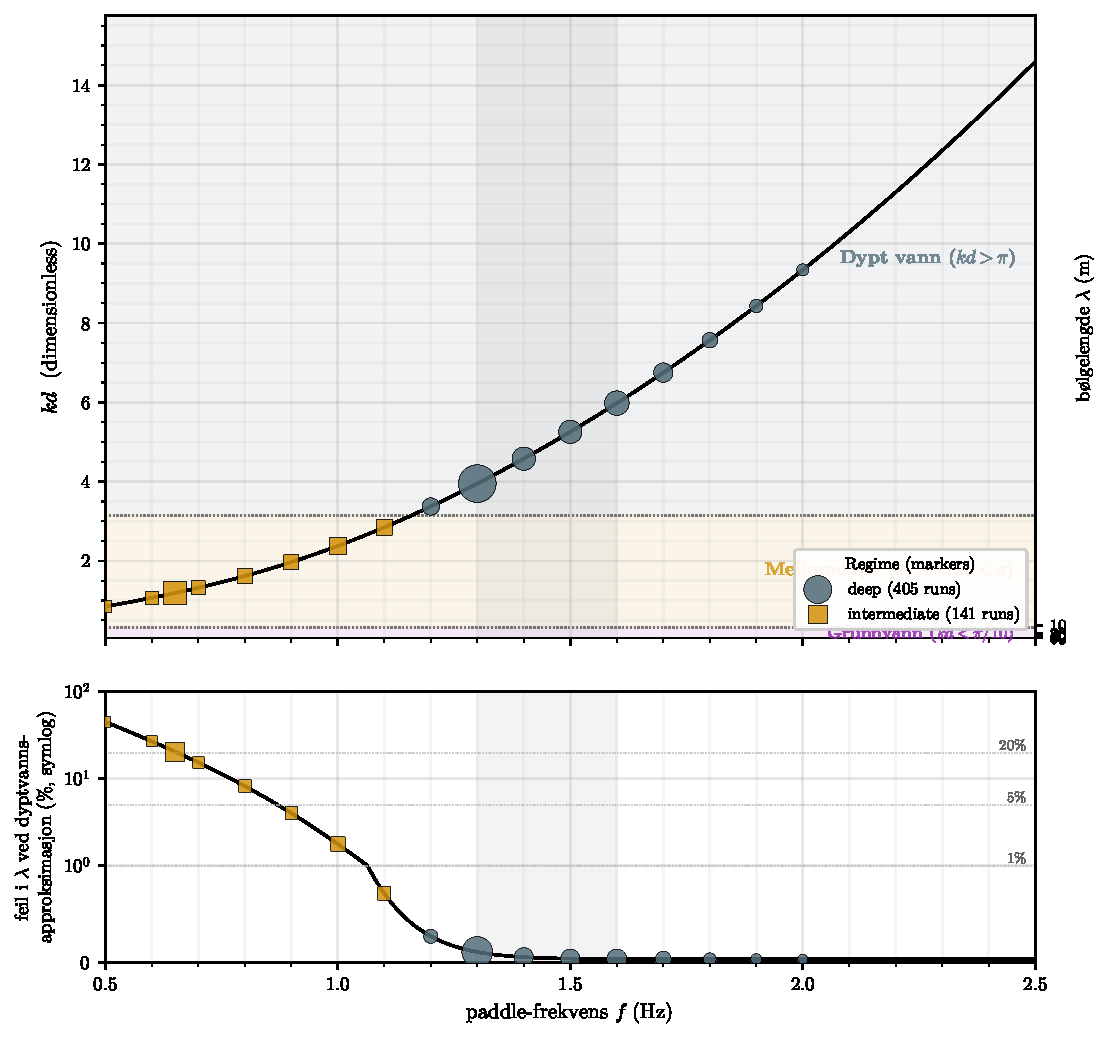
\includegraphics[width=\linewidth]{FIGURES/ch04_depth_regime.pdf}
  \caption{
    % TODO: write caption
  }
  \label{fig:ch04_depth_regime}
\end{figure}
